%<dscrpt>Déterminant d'une matrice aléatoire circulante.</dscrpt>
Dans tout le problème, $n$ désigne un entier naturel non nul et $\xi$ le complexe $\xi = e^{\frac{2i\pi}{n}}$. 

\subsection*{Partie I Calcul d'un déterminant circulant}

Soient $a_{0}, ..., a_{n-1}\in \C$ et $P$ le polynôme:
\[
P = \sum_{k=0}^{n-1}a_{k}X^{k} \in \C[X].
\]
Cette partie a pour but de calculer le déterminant de $C(a_{0}, ..., a_{n-1})$ défini par 
\[ 
C(a_{0}, ..., a_{n-1}) =\begin{pmatrix}
       a_{0} & a_{1} & a_{2} & \hdots & a_{n-1}\\
       a_{n-1}& a_{0} & a_{1} & & a_{n-2}\\
       a_{n-2} & a_{n-1} & a_{0} & & a_{n-3}\\
       \vdots & & & \ddots & \vdots \\
       a_{1} & a_{2} & a_{3} & \hdots & a_{0}
      \end{pmatrix}.
\]

\begin{enumerate}
 \item Notons $V = (\xi^{(j-1)(i-1)})_{(i, j)\in \llbracket 1, n\rrbracket^{2}}$:
            \[ V  = \begin{pmatrix}
                     1 & 1 & 1 & \hdots & 1\\
                     1 & \xi & \xi^{2} & \hdots & \xi^{n-1}\\
                     1 & \xi^{2} & \xi^{4} & \hdots & \xi^{2(n-1)}\\
                     \vdots & \vdots & \vdots & & \vdots \\
                     1 & \xi^{n-1} & \xi^{2(n-1)} & \hdots & \xi^{(n-1)(n-1)}
                    \end{pmatrix}\]
                    
 \begin{enumerate}
            \item Donner sans démonstration une expression de $\det(V)$.
            \item Soit $z_1, \cdots ,z_n$ des nombres complexes et $Q = (X-z_1) \cdots (X-z_n)$.\newline
Montrer que
\[
  \prod_{(i,j)\in \llbracket 1,n \rrbracket^{2} \atop i \neq j}(z_j - z_i)
  = \prod_{i \in \llbracket 1,n \rrbracket}Q'(z_i)
\]
\item En factorisant $X^{n}-1$, montrer que $\prod_{k=0}^{n-1}\xi^{k} = (-1)^{n-1}$.
\item En déduire que $\det(V) = \varepsilon n^{\frac{n}{2}}$ avec $\varepsilon \in\{ 1, -1, i, -i\}$.

\item Pour tout $p\in \llbracket 0, n-1\rrbracket$, notons:
 \[e_{p} = (1, \xi^{p}, \xi^{2p}, ..., \xi^{(n-1)p})\in \C^{n}. \]
 Montrer que la famille $(e_{0}, ..., e_{n-1})$ est une base de $\C^{n}$.
           \end{enumerate}

\item Pour tout $p\in \llbracket 0, n-1\rrbracket$, notons $E_{p}$ la matrice colonne représentant le vecteur $e_{p}$ dans la base canonique de $\C^{n}$:

 \[ E_{p} = \begin{pmatrix}
             1 \\ \xi^{p} \\ \xi^{2p} \\ \vdots \\ \xi^{p(n-1)}
            \end{pmatrix}\]
Montrer que $C(a_{0}, ..., a_{n-1})E_{p} = P(\xi^{p})E_{p}$.

\item Montrer que la matrice $C(a_{0}, ..., a_{n-1})$ est semblable à une matrice diagonale que l'on explicitera.

\item Montrer que:
\[ \det(C(a_{0}, ..., a_{n-1})) = \prod_{p=0}^{n-1}P(\xi^{p}).\]

\end{enumerate}


\subsection*{Partie II Combinaisons de racines de l'unité à coefficients aléatoires}

Soit $(\Omega, \p)$ un espace probabilisé fini, soient $X_{1}, ..., X_{n}$ des variables aléatoires définies sur $\Omega$ et à valeurs dans $\{ -1, 1 \}$, mutuellement indépendantes et telles que:
\[ \forall k\in \llbracket 1, n\rrbracket ,\ \p(X_{k} = 1) = \p(X_{k} = -1) = \frac{1}{2}.\]
Notons $Z:\Omega \to \C$ la variable aléatoire définie pour tout $\omega\in \Omega$ par:
\[ Z(\omega) = \sum_{k=1}^{n}X_{k}(\omega)e^{\frac{2ik\pi}{n}}.\]

Pour tout $k\in \N$, on notera $\abs{Z}^{k}$ la variable aléatoire définie pour tout $\omega \in \Omega$ par:
\[ \abs{Z}^{k}(\omega) = \abs{Z(\omega)}^{k}.\]

\begin{figure}[h!]
  \centering
  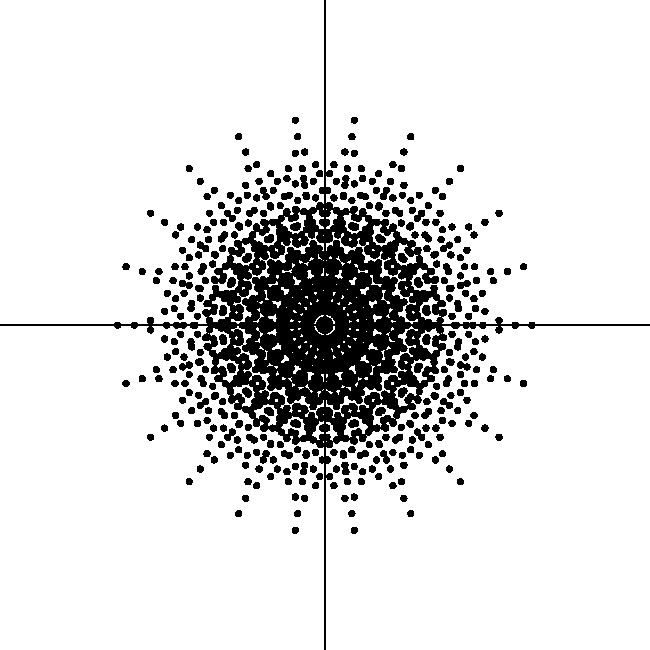
\includegraphics{Evaleadetcirc_1.pdf}
  % Cvaleadetcirc_1.pdf: 312x312 px, 72dpi, 11.01x11.01 cm, bb=0 0 312 312
  \caption{Valeurs de $Z$ pour $n=11$}
  \label{fig:Evaleadetcirc}
\end{figure}


\subsubsection*{II.1 Espérance et variance}

\begin{enumerate}

\item \begin{enumerate}
           \item Soient $1\leq k < l \leq n$. Donner la valeur de $\mathbb{E}(X_{k})$ puis de $\mathbb{E}(X_{k}X_{l})$.
           \item En déduire que $\mathbb{E}(\abs{Z}^{2}) = n$. 
          \end{enumerate}
          
\item \begin{enumerate}
           \item Soient $i,j,k,l\in \llbracket 1, n\rrbracket$ tels que $i < j$ et $k < l$. Montrer que $\mathbb{E}(X_{i}X_{j}X_{k}X_{l}) \neq 0$ si et seulement si $i = k$ et $j = l$.
           \item Calculer $\mathbb{E}(\abs{Z}^{4})$ puis $\mathbb{V}(\abs{Z}^{2})$.
          \end{enumerate}
\end{enumerate}


\subsubsection*{II.2 Inégalités de concentration.}

Dans toute cette partie, $t$ désigne un réel strictement positif.

\begin{enumerate}



\item Montrer que:
\[ \p(\abs{Z}^{2} \geq t) \leq \frac{n}{t}.\]

La suite de la partie II.2 est consacrée à la démonstration d'une meilleure majoration. Notons $X$ et $Y$ les variables aléatoires définies pour tout $\omega \in \Omega$ par:
\[ X(\omega) = \sum_{k=1}^{n}X_{k}\cos \left ( \frac{2k\pi}{n}\right ),\qquad Y(\omega) = \sum_{k=1}^{n}X_{k}\sin \left ( \frac{2k\pi}{n}\right ).\]

\item \begin{enumerate}
           \item Montrer que pour tout $x\in \R$, $\operatorname{ch}(x) \leq e^{\frac{x^{2}}{2}}$. 
           On pourra dériver deux fois la fonction $f:x\in \R \mapsto e^{-\frac{x^{2}}{2}}\operatorname{ch}(x)$.
           \item Calculer la somme:
           \[ \sum_{k=0}^{n-1}\cos^{2}\left ( \frac{2k\pi}{n}\right ).\]
           \item Montrer que pour tout $\theta \in \R$:
           \[ \mathbb{E}(e^{\theta X})\leq e^{\frac{n\theta^{2}}{4}}.\]
           
          \end{enumerate}
          
\item Montrer que pour tout $\theta \in \R_{+}$:
\[ \p (X \geq t) \leq e^{-\theta t + \frac{n\theta^{2}}{4}}.\]

\item En déduire que:
\[ \p(X \geq t) \leq e^{-\frac{t^{2}}{n}}.\]

\item Montrer que $X$ et $-X$ ont même loi et en déduire que:

\[ \p(\abs{X}\geq t) \leq 2e^{-\frac{t^{2}}{n}}.\]

On admet que pour tout $t\in \R^{+}$:
\[ \p(\abs{Y}\geq t) \leq 2e^{-\frac{t^{2}}{n}}.\]

\item Comparer les événements $\{ \abs{Z}^{2}\geq t \}$ et $\{ \abs{X} \geq \sqrt{\frac{t}{2}}\} \cup \{ \abs{Y} \geq \sqrt{\frac{t}{2}} \}$. En déduire que:
\[ \p(\abs{Z}^{2}\geq t) \leq 4e^{-\frac{t}{2n}}.\]

 
 

\end{enumerate}

\subsection*{Partie III. Déterminant d'une matrice circulante aléatoire}

Dans cette partie, {\bf l'entier $n$ est supposé premier impair}.\newline
On rappelle que $\mathbb{U}_{n}$ désigne l'ensemble des racines $n$-èmes de l'unité.\newline
On munit l'ensemble $\mathcal{P}(\mathbb{U}_{n})$ des parties de $\mathbb{U}_{n}$ de l'équiprobabilité $\p$.\newline
Pour tout $u\in \mathbb{U}_{n}$, on note $X_{u}:\Omega \to \{ -1, 1\}$ la variable aléatoire définie sur $\Omega$ par:
\[
\forall J\in \Omega,\ 
  X_{u}(J) = 
    \left \lbrace
      \begin{aligned}
         1 & \text{ si } u\in J\\
        -1 & \text{ si } u\not \in J 
      \end{aligned}
    \right.
\]

\begin{enumerate}
 \item 
  \begin{enumerate}
   \item Montrer que pour tout $u\in \mathbb{U}_{n}$:
 \[ \p(X_{u} = 1) = \p(X_{u} = -1) = \frac{1}{2}.\]
   \item Montrer que les variables aléatoires $X_{u}$ ($u\in \mathbb{U}_{n}$) sont mutuellement indépendantes. 
  \end{enumerate}

Pour tout $k\in \llbracket 0, n - 1\rrbracket$, notons $Z_{k} : \Omega \to \R_{+}$ la variable aléatoire définie pour tout $J \in \Omega$ par:
\[ Z_{k}(J) = \sum_{u\in \mathbb{U}_{n}}^{n}X_{u}(J)u^{k}.\]
Ainsi, la variable aléatoire $Z_{1}$ a la même loi que la variable aléatoire $Z$ définie dans la partie II.




 \item On rappelle que $n$ est premier. Soit $k\in \llbracket 1, n-1\rrbracket$. 
           \begin{enumerate}
            \item Montrer que l'application $\varphi_{k}: u\in \mathbb{U}_{n} \mapsto u^{k}\in \mathbb{U}_{n}$ est une bijection.
            
            On note $\overline{\varphi_{k}}: J\in \Omega \mapsto \varphi_{k}(J)\in \Omega$ la bijection qui à toute partie $J$ de $\mathcal{P}(\mathbb{U}_{n})$ associe son image directe par $\varphi_{k}$.
            \item Montrer que $Z_{k} = Z_{1}\circ \overline{\varphi_{k}}$.
            \item En déduire que $Z_{k}$ et $Z_{1}$ ont même loi.
           \end{enumerate}
           
On note $D:\Omega \to \R_{+}$ la variable aléatoire définie par:
\[ \forall J \in \Omega,\ D(J) = \abs{\det(C(X_{\xi^{0}}(J), X_{\xi^{1}}..., X_{\xi^{n-1}}(J)))}.\]

 \item Montrer à l'aide de la partie I que pour tout $J\in \Omega$:
 \[ D(J) = \abs{Z_{0}(J)}\prod_{k=1}^{\frac{n-1}{2}}\abs{Z_{k}(J)}^{2}.\]

 \item Posons $M:\Omega \to \R_{+}$ la variable aléatoire définie pour tout $J \in \Omega$ par:
 \[ M(J) = \max_{k\in \llbracket 1, \frac{n-1}{2}\rrbracket}\abs{Z_{k}(J)}^{2}.\]
 Montrer à l'aide de la partie II que pour tout $t\in \R_{+}$:
 \[ \p(M\geq t) \leq 2(n-1)e^{-\frac{t}{2n}}.\]
 
 
 \item Montrer que pour tout $t\in \R^{+}$:
 \[ \p(D\geq nt^{\frac{n-1}{2}}) \leq 2(n-1)e^{-\frac{t}{2n}}.\]
 
 \item Soit $W:\Omega \to \R^{+}$ une variable aléatoire, soit $p\in \N$ tel que $W(\Omega) \subset [ 0, p]$.
 \begin{enumerate}
  \item Montrer que:
  \[ \mathbb{E}(W) \leq \sum_{k=0}^{p}(k+1)(\p(W\geq k) - \p(W\geq k+1)).\]
  \item Montrer que:
  \[ \mathbb{E}(W) \leq 1 + \sum_{k=1}^{p}\p(W\geq k).\]
 \end{enumerate}
 
 
 \item \begin{enumerate}
            \item Montrer que $D(\Omega) \subset [ 0, n^{n}]$.
            \item Montrer que:
            \[ \mathbb{E}(D) \leq 1 + 2(n-1)\sum_{k=1}^{n^{n}}\exp\left ( -\frac{{\left (\frac{k}{n}\right )^{\frac{2}{n-1}}}}{2n}\right ).\]
            \item Montrer que pour tout $k\in \N$:
            \[ \int_{0}^{k/2}t^{k}e^{-t}\ dt \leq k!.\]
            \item Calculer l'intégrale:
            \[ \int_{0}^{n^{n}}\exp\left ( -\frac{{\left (\frac{x}{n}\right )^{\frac{2}{n-1}}}}{2n}\right )\ dx.\]
            \item En déduire que:
            \[ \mathbb{E}(D) \leq 1 + n\left [\left ( \frac{n-1}{2}\right )!\right ] (2n)^{\frac{n-1}{2}}.\]
           \end{enumerate}


 


 
\end{enumerate}

